\section{Dimension of $\mathbf{w}$}
Suppose we are given a data set $\mathfrak{D}$,
\[\mathfrak{D} = \{(x_i,y_i) \mid i \in [|\mathfrak{D}|], x_i \in \mathbb{R}, y_i \in \mathbb{R}\}\]
where, $[n] := \{1,2, \dots n\} \forall n \in \mathbb{N}$. Denote,
\[\mathfrak{D}\mid_x := \{x_i \mid (x_i,y_i) \in \mathfrak{D}\}\]
\[\mathfrak{D}\mid_y := \{y_i \mid (x_i,y_i) \in \mathfrak{D}\}\]
\\ 
Further suppose that the data set is distributed around some line given by $y = mx + c$.
That is, \[y_i = mx_i + c + \epsilon_i \text{ } \forall i \in [|\mathfrak{D}|]\]
where $\epsilon_i \sim \mathbb{P}(\cdot)$. Thus we have the following picture,
\begin{figure}[h]
    \centering
    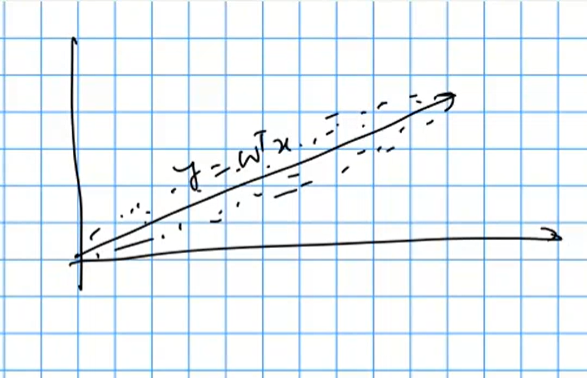
\includegraphics[height = 5cm, width = 5cm]{pictures/q4.PNG}
    \caption{A picture of the data}
\end{figure}


Now, for each $x_i \in \mathfrak{D}\mid_x$, and for all $n \in \mathbb{N}$, define,
\[\mathbf{x}_i := (x_i,x_i^2 \dots x_i^n)^T \in \mathbb{R}^n\]
Further, let $\mathbf{w} \in \mathbb{R}^n$. We ask the following question,
\begin{center}
    \underline{Question} What is the $n$, such that we can be \textit{assured} that the following holds: 
    \[y_i = \mathbf{w}^T\mathbf{x}_i \forall y_i \in \mathfrak{D}_y\]
\end{center}
Informally, in the extreme overfitting case, what is the minimum error that we get -- and what is the corresponding dimension of the weights vector, that is $n$?

Note the following lemma.
\begin{lemma}
Given $n+1$ points $(x_i,y_i)$ with $n \geq 1$, such that all the $x_i$ are distinct. There exists a $n$ degree polynomial $p$ with coefficients $(a_n,a_{n-1}, \dots a_0)$ such that
\[p(x_i) = y_i \forall i \in [n+1]\]
\end{lemma}
\begin{proof}
We have the following equations,
\[a_nx_i^n + a_{n-1}x_i^{n-1} + \dots a_0 = y_i \forall i \in [n+1]\]
This can be expressed in the matrix form as,
\[\begin{pmatrix} x_1^n & x_1^{n-1} & \dots &x_1& 1 \\ 
\vdots & \vdots & \ddots &\vdots&\vdots \\  x_{n+1}^n & x_{n+1}^{n-1} & \dots &x_{n+1}& 1
\end{pmatrix} \begin{pmatrix} a_n \\ a_{n-1} \\ \vdots \\ a_0 \end{pmatrix} = \begin{pmatrix}y_{0} \\ y_1 \\ \vdots \\ y_{n+1}\end{pmatrix}
\]
Note that the matrix on the left is a Vandermonde matrix, and has a non zero determinant. Thus the system of equations has a unique solution.
\end{proof}


For our case, since we do not have a bias term (note the definition of $\mathbf{x}_i$), our equations would be of the form,
\[a_nx_i^n + a_{n-1}x_i^{n-1} + \dots + a_1x_i = y_i\]
Thus (assume non zero $x_i$), 
\[a_nx_i^{n-1} + a_{n-1}x^{n-2} + \dots + a_1 = y_i/x_i\]
By the previous lemma, we have,
\[n - 1 = |\mathfrak{D}| - 1\]
Thus, \[n = |\mathfrak{D}|\]
Thus, we should have,
\[\text{dim}(\mathbf{w}) \leq |\mathfrak{D}|\]
\hfill\qedsymbol


But, this says that the number of parameters is dependent on the number of features! This should not be the case! \\ 
Interestingly, in deep learning, networks are more often than not extremely overparametrised (look up some typical neural nets) - and still we obtain good generalization errors! So, even with a \textit{lot} of parameters \textit{without} regularization, the deep learning model will ``understand" the situation and put certain weights to zero!

